\documentclass{llncs}
\usepackage[utf8]{inputenc}
\usepackage{verbatim}
\usepackage{multicol}
\usepackage{llncsdoc}
\usepackage{amsmath}
\usepackage{amsfonts}
\usepackage{amssymb}
\usepackage{graphicx}
\usepackage{lmodern}
\usepackage{calc}
\usepackage{enumitem}
\usepackage{algpseudocode}
\usepackage{algorithm}
\usepackage{algorithmicx}

\algsetblockdefx[IfContinue]{IfContinue}{IfContinue}
{0}{0pt}
[0]{}
[1]{\textbf{if} #1 \textbf{continue}}

\algrenewcommand\algorithmicrequire{%
  \makebox[\widthof{\textbf{Output:}}][l]{\textbf{Input:}}}
  
 \algrenewcommand\algorithmicensure{%
  \textbf{Output:}}

\usepackage{color}
\usepackage{gnuplottex}
\usepackage{subcaption}
\usepackage{microtype}
\usepackage[normalem]{ulem}
\captionsetup{compatibility=false}
\usepackage{tikz}
\usetikzlibrary{trees,automata,positioning}
\usepackage{booktabs}
\usepackage{gnuplottex}
\usepackage{xparse}
\usepackage{epstopdf}
% For scaling gnuplottex
\ExplSyntaxOn
\DeclareExpandableDocumentCommand{\convertlen}{ O{cm} m }
 {
  \dim_to_unit:nn { #2 } { 1 #1 } cm
 }
\ExplSyntaxOff

%% For lattice figure
% Set the overall layout of the tree
\tikzstyle{level 1}=[level distance=3.0cm, sibling distance=0.6cm]
\tikzstyle{level 2}=[level distance=3.5cm, sibling distance=0.6cm]
\tikzstyle{level 3}=[level distance=3.5cm, sibling distance=0.6cm]

% Define styles for bags and leafs
\tikzstyle{l1} = [rectangle, text width=5em, text centered]
\tikzstyle{l2} = [rectangle, text width=5em, text centered]
\tikzstyle{l3} = [rectangle, text width=5em, text centered]

% only when using asmthm
%\newtheorem{definition}{Definition}
%\newtheorem{theorem}{Theorem}

\author{Micky Faas \and Matthijs van Leeuwen}
\title{VOUW: Geometric Pattern Mining using the MDL Principle}
\institute{Leiden Institute for Advances Computer Science}
\begin{document}

\section{Theoretical Framework}

%\subsection{On Patterns and Matrices}

%In this subsection we will introduce a method for describing and decomposing tabular or matrix-like data. It is this concise notation that allows us to reason about what one can and cannot expect to find from a set of data and what this data could look like. In later subsections we will use these tools to gradually connect to the MDL principle and finally to a practical search algorithm.

We define geometric pattern mining on bounded, discrete and two-dimensional raster-based data. We represent this data as an $M\times N$ matrix $A$ whose rows and columns are finite and in a fixed ordering (i.e. reordering rows and columns semantically alters the matrix). For elements $a_{i,j}$, where row $i$ is on $[0;N)$ and column $j$ is on $[0;M)$, holds that $a_{i,j} \in S$, the finite set of symbols occurring in $A$. %We will denote $A$ as a matrix because of the convenience of the linear algebra notation\footnote{In any practical application however, $A$ will not represent a system of linear equations but rather hold some form of sampled data that can be placed on a grid.}

\begin{figure}

\small
$$
A =
\begin{bmatrix}
1 & \cdot & \cdot & \cdot & 1 & 1 &  \\[-.2em]
\cdot & 1 & \cdot & \cdot & \cdot & \cdot &  \\[-.2em]
1 & \cdot & \cdot & \cdot & 1 & \cdot &  \\[-.2em]
\cdot & 1 & \cdot & \cdot & \cdot & 1 &  \\[-.2em]
1 & 1 & 1 & 1 & \cdot & \cdot &  \\
\end{bmatrix}\!\!, \
I = 
\begin{bmatrix}
X & \cdot & \cdot & \cdot & Y & \cdot & \\[-.2em]
\cdot & \cdot & \cdot & \cdot & \cdot & \cdot &  \\[-.2em]
X & \cdot & \cdot & \cdot & X & \cdot &  \\[-.2em]
\cdot & \cdot & \cdot & \cdot & \cdot & \cdot &  \\[-.2em]
Y & \cdot & Y & \cdot & \cdot & \cdot &  \\[-.2em]
\end{bmatrix}\!\!, \
H = \left\{
X =
\begin{bmatrix}
1 & \cdot \\[-.2em]
\cdot & 1
\end{bmatrix}\!\!,
Y =
\begin{bmatrix}
1 & 1
\end{bmatrix}\right\}
$$
\caption{Example decomposition of $A$ into instantiation $I$ and patterns $X,Y$.}

\label{example1}
\end{figure}

According to MDL, the shortest (optimal) description of $A$ reveals all structure of $A$ in the most succinct way possible and we approximate this optimal description through the compression of the original data. This optimal description $A'$ is only optimal if we can unambiguously reconstruct $A$ from it and nothing more --- the compression is both minimal and lossless. Intuitively compression means defining $A$ using as few building blocks as possible. We illustrate this in Figure \ref{example1}. Given the matrix $A$ we decompose it in patterns, denoted $X$ and $Y$. The set of all these patterns is the \textbf{model} of a $A$, denoted $H_A$. In order to reconstruct $A$ from this model, we alse need a mapping from the $H_A$ back to $A$. This mapping represents in what MDL calls the \textbf{the data given the model $H_A$}. In this context we think of it as `instructions' of how to reconstruct $A$. Let us call the set of all instructions required to rebuild $A$ from $H_A$ the \textbf{instantiation} of $H_A$. It is denoted by ${I}_A$ in the example.  The result is a notation that allows us to express matrix $A$ as if decomposed into sets of local and global spatial information, which we will now describe in more detail.

% Notice how $I_A$ essentially tells us where in $A$ each pattern from $H_A$ was originally located.

%We call a specific set of patterns $H\in \mathcal{H}_A$ a \textbf{point hypothesis} and analogously a specific instantiation is denoted ${I} \in \mathcal{I}_A$. Formally, a complete description $A'$ of $A$ is a combination of some $H$ and ${I}$ such that ${I}$ is a 1-to-1 mapping from $H_A$ to $A$. In the next subsections we will formalize these concepts by starting bottom-up with patterns and instances up to models, instantiation matrices and their link with MDL. After this we will discuss how we propose to find a good description of $A$ by means of the VOUW algorithm.


\subsection{Patterns and Instances}
\noindent $\triangleright$ \emph{We define a \textbf{pattern} as a $M_X\times N_X$ submatrix $X$ of the original matrix $A$. Elements of this submatrix may be $\cdot$, the empty element, which gives us the ability to cut-out any irregular-shaped part of $A$. We additionally require the elements of $X$ to be adjacent (horizontal, vertical or diagonal) to at least one non-empty element and that no rows and columns are empty.}
%While this limits the amount of possible patterns somewhat, it will later on also reduce the computational effort dramatically.
%We will now define a pattern to be the smallest submatrix to completely contain all elements of $X$.

%\begin{definition}
%A \textbf{pattern} $X$ is a $M_X\times N_X$ submatrix of $A$ where any non-empty element may %optionally be replaced by $\cdot$ such that:
%\begin{itemize}
%\item Any non-empty element in $X$ is adjacent (horizontal, vertical or diagonal) to at least one other non-%empty element.
%\item The first and last rows and columns contain at least one non-empty element.
%\end{itemize}
%\end{definition}
\smallskip

From this definition, the dimensions $M_X\times N_X$ give the smallest rectangle around $X$ (the \emph{bounding box)}. We also define the cardinality $|X|$ of $X$ as the number of non-empty elements. We call a pattern $X$ with $|X|=1$ a \textbf{singleton pattern}, i.e. a pattern containing exactly one element of $A$. %\footnote{We will often slightly abuse notation by using single-index elements or using set notation for any matrix. For instance, when we write $x_i \in X$, we mean that $x_i$ is the $i$-th non-empty element in $X$ with $1\leq i \leq |X|$. By convention we will always use row-major ordering in these cases.}

Each pattern contains a special \textbf{pivot} element: %
%\begin{definition}
$pivot(X)$ is the first non-empty element of $X$. % in the first non-empty column of the first (non-empty) row of $X$.
%\end{definition}
\noindent
A pivot can be thought of as a fixed point in $X$ which we can use to position its elements in relation to $A$. This translation, or \textbf{offset}, is a tuple ${q}=(i,j)$ that is on the same domain as an index in $A$. We realize this translation by placing all elements of $X$ on an empty $M\times X$ size matrix in such that the pivot element is at $(i,j)$. We formalize this in the \textbf{instantiation operator} $\otimes$:

\smallskip
\noindent $\triangleright$
%\begin{definition}
%In the context of an $M\times N$ matrix $A$,
\emph{We define the \textbf{instance} $X \otimes {(i,j)}$ as the $M\times N$ matrix containing all elements of $X$ such that $\mathrm{pivot}(X)$ is at index $(i,j)$ and the distances between all elements are preserved. The resulting matrix contains no additional non-empty elements. } %
%\end{definition}
\smallskip

%So according to this definition $\otimes$ adds `padding' around the elements of a pattern to align its pivot to a certain offset $(i,j)$. 
Obviously this does not yield a valid result for an arbitrary offset $(i,j)$. We want to limit ourselves to the space of pattern instances that are actually valid in relation to matrix $A$. Therefore two simple constraints are needed: (1) an instance must be \textbf{well-defined}: \emph{placing $\mathrm{pivot}(X)$ is at index $(i,j)$ results in an instance that contains all elements of $X$, and (2) elements of instances cannot overlap, meaning each element of $A$ should be described at most once.} This allows for a description that is both unambiguous and minimal.

\smallskip
%\begin{definition}
\noindent $\triangleright$
\emph{Two pattern instances $X \otimes {q}$ and $Y \otimes {r}$, with ${q} \neq {r}$ are \textbf{non-overlapping} if $|(X \otimes {q}) + (Y \otimes {r})| = |X|+|Y|$.}
%\end{definition}
\smallskip

From here on we will use the same letter in lower case to denote an arbitrary instance of a pattern, e.g. $x = X \otimes {q}$ when the exact value of ${q}$ is unimportant.%

We briefly introduced the instantiation $I$ as a set of `instructions' of where instances of each pattern should be positioned in order to obtain $A$. As Figure \ref{example1} suggests, this mapping has the shape of an $M\times N$ matrix.

\smallskip
%\begin{definition}
\noindent $\triangleright$
\emph{Given the set of patterns $H$, the \textbf{instantiation (matrix)} ${I}$ is an incomplete $M\times N$ matrix such that ${I}_{i,j} \in H \cup \{\cdot\}$ for all $(i,j)$. For all non-empty elements ${I}_{i,j}$ it holds that ${I}_{i,j} \otimes (i,j)$ is a non-overlapping instance of ${I}_{i,j}$ in $A$.}
%\end{definition}
\smallskip

The above definition creates the interesting proposition that the offset to each instance is unique. We provide a sketch proof in Appendix A.
%Given that a pattern's pivot is placed exactly at one offset and that instances must be non-overlapping, makes this indeed believable. Later when we inductively define the set $\mathcal{I}$ of all instantiation matrices, this will be shown to be true more formally. 

%%
%% Removing this for now...
\begin{comment}
\subsection{Geometries}

In the previous subsections we silently omitted an important constraint in instantiating patterns. An instance has only meaning in the context of matrix $A$ if their respective elements match. In order words, if an instance $X \otimes (i,j)$ has all its non-empty elements identical to the corresponding indices in $A$, this means that pattern $X$ matches $A$ in $(i,j)$. In this case the match is exact, formally
\begin{definition}
The instance ${x}=X \otimes {q}$ is an \textbf{exact match on $A$} if for all non-empty ${x}_{i,j} \in {x}$ it holds that ${x}_{i,j} = a_{i,j}$.
\end{definition}

While this form of straightforward matching can be desirable in some cases, it may lead to a bloated model in others. Take the example from Figure \ref{example3} that lists matrix $A$ and four patterns. Pattern $W$ is obviously an exact match to five of the six elements of $A$. Pattern $X$, while not an exact match, is also a good candidate to describe $A$ although it is multiplied by a constant factor of two. Pattern $Y$ is a near-exact match: only one element is off - this could be due to noise for example. Pattern $Z$ is no match for the values in $A$, but notice that it is identical in structure to the other patterns: it places as many values at the same indices. 

\begin{figure}
\tiny
$$
\left.
A =
\begin{bmatrix}
1 & 2 \\[-.2em]
\cdot & 1 \\[-.2em]
1 & 2
\end{bmatrix}\
\right\rvert
W =
\begin{bmatrix}
1 & 2 \\[-.2em]
\cdot & 1 \\[-.2em]
1 & 2
\end{bmatrix}\!\!,
$$
$$
X =
\begin{bmatrix}
2 & 4 \\[-.2em]
\cdot & 2 \\[-.2em]
2 & 4
\end{bmatrix}\!\!,
Y =
\begin{bmatrix}
1 & 2 \\[-.2em]
\cdot & 1 \\[-.2em]
1 & 1
\end{bmatrix}\!\!,
Z =
\begin{bmatrix}
2 & 2 \\[-.2em]
\cdot & 0 \\[-.2em]
4 & 3
\end{bmatrix}\!\!,
$$
\caption{Examples of structurally equivalent patterns with varying degrees of similarity.}

\label{example3}
\end{figure}

The example above suggests that we could do one more step of decomposition: just like we decomposed the original matrix into global structure (instantiation) and local structure (pattern), we decompose patterns into structure and magnitude. 

\begin{definition}
The \textbf{geometry} $G(X)$ of pattern $X$ is an equally-sized Boolean matrix such that $G(X)_{i,j}=1$ whenever $X_{i,j}$ is non-empty.\\
The \textbf{magnitude} $M(X)$ of pattern $X$ is the string of values obtained by taking each non-empty element of $X$ in row-major order.
\end{definition}

In the example we can see that $G(X)= \tiny\begin{bmatrix}1 & 1 \\[-.2em]\cdot & 1 \\[-.2em]1 & 1\end{bmatrix}$ and that $M(X)=1\ 2\ 1\ 1\ 2$. In fact, because all four patterns have the same geometry, we say that they are \textbf{isomorphic}. As such we write $X \cong Y$ iff $G(X) = G(Y)$. 

To understand the importance of separating the structure and magnitude of patterns, let us briefly expand the example above. Suppose we have a large matrix $B$ that consists of $n$ clusters of matrices $W$ and $X$ from Figure \ref{example3}. To determine the optimal description of $B$, we might want to look at the prevalence of each submatrix. Say it contains $\frac{n}{2}$ $W$'s and $\frac{n}{2}$ $X$'s. In this case it makes sense to include both patterns in the description. However, we could also exploit the fact that the structure of both patterns is equivalent and make the description more concise by only storing $G(W)$ and then $M(W)$ and $M(X)$ separately. Now imagine that $B$ only contains one $W$ and $n-1$ $X$'s. In this case the one $W$ might be an anomaly that we would like to detect. However, it could also be due to noise in the data in which case we would like to describe $B$ just using $n$ $X$'s. It is impossible to make this distinction beforehand. 

One possibility for solving this problem is to let the MDL equation decide whether the stray $W$ is an anomaly or not. Recall that according to the MDL principle the most succinct description is the best. Therefore if the amount of `effort' required to transform $X$ into $W$ is small, we should probably encode that one $W$ using $X$. In that case it is considered noise, while it is probably an anomaly if doing so would yield a larger description.
\end{comment}
%%%
%%%
\subsection{The Problem and its Solution Space}

%\subsubsection{Constructing Patterns}
\label{constructpatterns}
%Patterns can be joined to create increasingly large patterns and, as we will later see, this concept forms the basis of the search algorithm. However, two patterns could be joined in any different number of ways.

Patterns can be constructed by joining smaller patterns in a bottom-up fashion. We can define the exact way two patterns should be joined by enumerating the distance of their respective pivots. To limit the possibilities to patterns relevant to $A$, instances can be used as an intermediate step. Since instances are simply patterns projected on an $M\times N$ matrix, we can reverse $\otimes$ by removing all completely empty rows and columns:

\smallskip
\noindent $\triangleright$
%\begin{definition}
\emph{Let $X \otimes {q}$ be an instance of $X$, then by definition we say that $\oslash(X \otimes {q}) = X$.}
%\end{definition}
\smallskip

As Figure \ref{example2} demonstrates, we can use a simple element-wise matrix addition to sum two instances and use $\oslash$ to obtain a joined pattern. Here we start by instantiating $X$ and $Y$ with offsets $(1,0)$ and $(1,1)$ respectively. We add the resulting ${x}$ and ${y}$ to obtain $\oslash{z}$, the union of $X$ and $Y$ with relative offset $(1,1)-(1,0)=(0,1)$. %We formally describe this mechanism in Theorem \ref{fundamental}. As we will see later, this will become the fundamental operation of our algorithm.

\begin{figure}[b]
\centering
\small
$$
X =
\begin{bmatrix}
1 & \cdot \\[-.2em]
\cdot & 1
\end{bmatrix}\!\!,
Y =
\begin{bmatrix}
1
\end{bmatrix}\!\!,
$$
$$
\bar{X} = X\oplus (1,0) =
\begin{bmatrix}
\cdot & \cdot \\[-.2em]
1 & \cdot \\[-.2em]
\cdot & 1
\end{bmatrix}\!\!,
$$
$$
\bar{Y} = Y\oplus (1,1) =
\begin{bmatrix}
\cdot & \cdot \\[-.2em]
\cdot & 1 \\[-.2em]
\cdot & \cdot
\end{bmatrix}\!\!,
$$
$$
\bar{X} + \bar{Y} =
\begin{bmatrix}
\cdot & \cdot \\[-.2em]
1 & 1 \\[-.2em]
\cdot & 1
\end{bmatrix}\!\!,
$$
$$
Z = \ominus(\bar{X}+\bar{Y})=
\begin{bmatrix}
1 & 1 \\[-.2em]
\cdot & 1
\end{bmatrix}\!\!
$$
\caption{Example of Theorem \ref{fundamental}. The $2\times 3$ input matrix is not shown.}
\label{example2}
\end{figure}

\begin{theorem}\label{fundamental}
Given two non-overlapping instances ${x}=X\otimes {q}$ and ${y}=Y\otimes {r}$, the sum of the matrices ${x} + {y}$ is another instance. We observe that pattern $Z=\oslash({x} + {y})$ such that ${x} + {y} = Z\otimes {q}$.
\end{theorem}

%Notice that this sum has the limitation that two instances can only be summed if they do not overlap. While this is a serious limitation, we will show in the next subsection that it is not of any practical relevance.


\subsubsection{The Sets $\mathcal{H}_A$ and $\mathcal{I}_A$}\label{thesetH}

%In the previous subsections we have given a means to describe a matrix $A$ in a different way, namely by means of patterns and instances. If we succeed in describing $A$, using our notation, in a more concise way than just $A$ itself, we have learned something about the local and global structure of $A$ and perhaps even about anomalies or noisy values. In this context, we see a clear relation the MDL principle and learning. 
%In order to find a short(er) description, we will first have to define our search space and the way solutions are to be constructed. 

We define the \textbf{model class} $\mathcal{H}$, the set of all possible models for all possible inputs. Without any prior knowledge, this is the search space of our algorithm. We will first look at a more bounded subset $\mathcal{H}_A$ of all possible models for $A$, and $\mathcal{I}_A$, the set of all possible instantiations to these models. We will also take $H_A^0$ to be the model with only singleton patterns. As singletons are just individual elements of $A$, we can simply say that $H_A^0=S$. The instantiation matrix corresponding to $H_A^0$ is denoted ${I}_A^0$. Given that each element of this matrix must correspond to exactly one element of $A$ in $H_A^0$, we see that each ${I}_{i,j} = a_{i,j}$ and so ${I}_A^0$ is equal to $A$. 

Using $H_A^0$ and ${I}_A^0$ as base cases we can now inductively define the set $\mathcal{I}_A$: % of all instantiations of all models over $A$:\\
\begin{description}[labelwidth=\widthof{\bfseries By induction}]
\item[Base case] ${I}_A^0 \in \mathcal{I}_A$
\item[By induction] If ${I}$ is in $\mathcal{I}_A$ then take any pair ${I}_{i,j},{I}_{k,l} \in {I}$ such that $(i,j)\leq(k,l)$ in lexicographical order. Then the set ${I}'$ is also in $\mathcal{I}_A$, providing ${I}'$ equals ${I}$ except:
\vspace{-1.5\baselineskip}
\begin{align*}
{I}_{i,j}' &:= \oslash \big( {I}_{i,j} \otimes (i,j) + {I}_{k,l} \otimes (k,l) \big) \\
{I}_{k,l}' &:= \cdot %\\
%{I}_{m,n}' &:= I_{m,n} \ \forall (m,n) \neq (i,j) \ \land \ (m,n) \neq (k,l)
\end{align*}
\end{description}

\noindent This shows we can add any two instances together, which are by definition always non-overlapping and thus valid in $A$, in any order and obtain an element of $\mathcal{I}_A$. Eventually this results in just one big instance that is equal to $A$. Note that when we take two elements ${I}_{i,j},{I}_{k,l} \in {I}$ we force $(i,j)\leq(k,l)$, not only to eliminate different routes to the same instance matrix, but also such that the pivot of the new pattern coincides with ${I}_{i,j}$. We can then leave ${I}_{k,l}$ empty.

The construction of $\mathcal{I}_A$ also implicitly defines $\mathcal{H}_A$. While this may seem odd --- defining models for instantiations instead of the other way around --- note that there is no unambiguous way to find one instantiation for a given model. Instead we find the following definition by applying the inductive construction:
% \footnote{Notice that this is a problem for any real-world implementation. We will describe a heuristic to derive instantiation matrices from model and data in the next section.}.
%
%\noindent $\triangleright$
%\begin{definition}
%\emph{The set $\mathcal{H}_A$ of all models over $A$ is given by:}
\begin{align}
\mathcal{H}_A=\big\{\{\oslash({I}) \ | \ {I} \in {I} \} \ \big | \ {I} \in \mathcal{I}_A \big\}.
\end{align}
%\end{definition}

\noindent So for any instantiation ${I}\in \mathcal{I}_A$ there is a corresponding set in $\mathcal{H}_A$ of all patterns that occur in ${I}$. This results in an interesting symbiosis between model and instantiation: increasing the complexity of one decreases that of the other. This construction gives a tightly connected lattice as shown in Figure \ref{lattice}. 
%\begin{theorem}
%Given any instantiation ${I}\in \mathcal{I}_A$ and its corresponding model in $%\mathcal{H}_A$, the matrix $A$ can be reconstructed unambiguously.
%\end{theorem}

\begin{figure}[t]
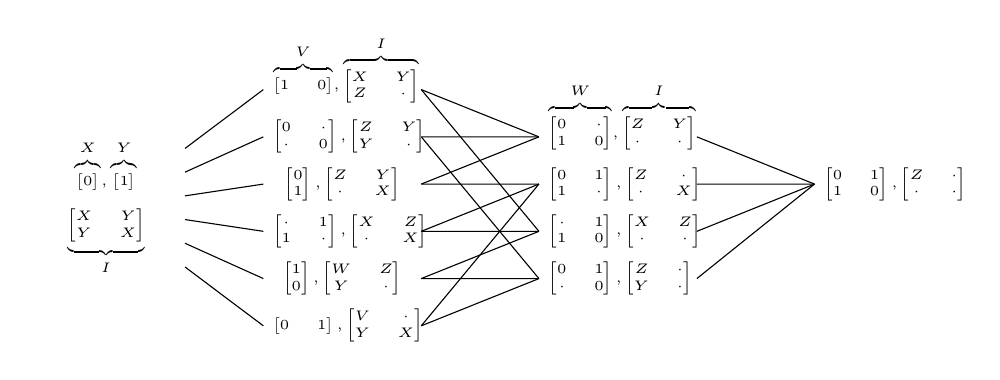
\begin{tikzpicture}[on grid, grow=right]
\node(R)[l1] {\tiny $\begin{matrix}\overbrace{\begin{bmatrix}0\end{bmatrix}}^{X},\overbrace{\begin{bmatrix}1\end{bmatrix}}^{Y}\\[1em]\underbrace{\begin{bmatrix}X & Y \\Y & X\end{bmatrix}}_{I}\end{matrix}$}
	child {
        node(F)[l3] {\tiny $\begin{bmatrix}0 & 1\end{bmatrix},\begin{bmatrix}V & \cdot \\Y & X\end{bmatrix}$}        
            edge from parent[draw=none] 
            (R) edge (F.west)
    }
    child {
        node(E)[l2] {\tiny $\begin{bmatrix}1 \\ 0\end{bmatrix},\begin{bmatrix}W & Z \\ Y & \cdot\end{bmatrix}$}        
            child {
                node(J)[l3]
                    {\tiny $\begin{bmatrix}0 & 1 \\ \cdot & 0\end{bmatrix},\begin{bmatrix}Z & \cdot \\ Y & \cdot\end{bmatrix}$}
                edge from parent 
            }
            edge from parent[draw=none] 
            (R) edge (E.west)
    }    
    child {
        node(D)[l2] {\tiny $\begin{bmatrix}\cdot & 1 \\ 1 & \cdot\end{bmatrix},\begin{bmatrix}X & Z \\ \cdot & X\end{bmatrix}$}        
            child {
                node(I)[l3]
                    {\tiny $\begin{bmatrix}\cdot & 1 \\ 1 & 0\end{bmatrix},\begin{bmatrix}X & Z \\ \cdot & \cdot\end{bmatrix}$}
                edge from parent 
            }
            edge from parent[draw=none] 
            (R) edge (D.west)
    }    
    child {
        node(C)[l2] {\tiny $\begin{bmatrix}0 \\ 1\end{bmatrix},\begin{bmatrix}Z & Y \\\cdot & X\end{bmatrix}$}        
            child {
                node(H)[l3]
                    {\tiny $\begin{bmatrix}0 & 1 \\ 1 & \cdot\end{bmatrix},\begin{bmatrix}Z & \cdot \\ \cdot & X\end{bmatrix}$
                    }                    
                    	child {
                    		node(K)[l3] {\tiny $\begin{bmatrix}0 & 1 \\ 1 & 0\end{bmatrix},\begin{bmatrix}Z & \cdot \\ \cdot & \cdot\end{bmatrix}$}
                    	}
                edge from parent 
            }
            edge from parent[draw=none] 
            (R) edge (C.west)
    }    
    child {
        node(B)[l2] {\tiny $\begin{bmatrix}0 & \cdot \\ \cdot & 0\end{bmatrix},\begin{bmatrix}Z & Y \\Y & \cdot\end{bmatrix}$}        
            child {
                node(G)[l3]
                    {\tiny $\overbrace{\begin{bmatrix}0 & \cdot \\ 1 & 0\end{bmatrix}}^{W},\overbrace{\begin{bmatrix}Z & Y \\ \cdot & \cdot\end{bmatrix}}^{I}$\vspace{.5cm}}
                edge from parent 
            }
            edge from parent[draw=none] 
            (R) edge (B.west)
    } 
    child {
        node(A)[l2] {\vspace{.5cm}\tiny $\overbrace{\begin{bmatrix}1 &0\end{bmatrix}}^{V},\overbrace{\begin{bmatrix}X & Y \\Z & \cdot\end{bmatrix}}^{I}$}        
        	edge from parent[draw=none] 
            (R) edge (A.west)
    };
\draw(F.east)--(H.west);
\draw(F.east)--(J.west);
\draw(B.east)--(J.west);
\draw(C.east)--(G.west);
\draw(D.east)--(H.west);
\draw(E.east)--(I.west);
\draw(A.east)--(G.west);
\draw(A.east)--(I.west);
\draw(G.east)--(K.west);
\draw(I.east)--(K.west);
\draw(J.east)--(K.west);
\end{tikzpicture}
\caption{Model space lattice for a $2\times 2$ Boolean matrix. The Left hand column shows which pattern is added in each step, $I$ is the current instantiation.}
\label{lattice}
\end{figure}

%\subsubsection{The Optimal Model}

%The final step in the process of describing $A$ is to select the `best' or `most optimal' model from the set of $\mathcal{H}_A$. While intuitively we can understand that not every model we pick is equally fitting in terms of how well it describes $A$, this concepts needs to be formalized before we can even begin to search $\mathcal{H}_A$. To this end we make the connection with the MDL principle that says, informally, that the most concise encoding of the data gives us the best description. Since we are using two-part MDL, it is very convenient that we have already split the problem into two parts:  a model $H_A$ and an instantiation ${I}_A$. Together they form $A'$ and according to MDL, their sum must be minimized. The two-part MDL equation is given by:
%$$
%L_1(H_A) + L_2(A|H_A)
%$$
%Here the functions $L_1, L_2$ are two independent length functions that make up the coding scheme for two-part MDL. This minimization is often thought of as compression, although we will not actually write any encoded data. This leaves us with the task of finding an encoding scheme that encodes both model and instantiations lossless and without redundancy.

%Say we have some set of code words $\{C_0,C_1,\dots,C_n\}$. These symbols could be for example be a code word for each pattern $X_0, X_1,\dots,X_n$ in a model. We now want to find optimal lengths $l_0,l_1,\dots,l_n$ to assign to each code word using the Kraft-inequality such that holds that $\displaystyle\sum^N_{i=0}r^{-l_i} \leq 1$. In this case we say that $r=2$ (symbols 0 and 1), so we can measure code lengths in bits. 
%The Kraft-inequality gives us a bijection between code lengths and probability distributions. This is one of the main ideas of Shannon's entropy, which plays also an important role in the MDL principle. In our example we can write a probability distribution $P(X)$ for $X \in H_A$, as the probability of pattern $X$ occurring in our instance set. Given these probabilities we can use $l_i=-\log(P(X_i))$ to compute the exact number of bits a pattern should optimally be encoded with\footnote{Notice how common code words are shorter then rarely used code words. According to the Kraft inequality this gives us an optimal code. The number of bits we compute are real numbers and not integers. While this does certainly not result in a practical encoding, for the purpose of model selection we do not actually need to encode the data as we are only interested in its hypothetical length.}.

\subsection{Encoding Models and Instances}

From all parametrized models in $\mathcal{H}_A$ we want to select (approximate) the model that describes $A$ best. We use two-part MDL to quantify how well a given model and instantiation matrix fit $A$. Two-part MDL tells us to minimize the sum of $L_1(H_A) + L_2(A|H_A)$, two functions that give the length of the model and the length of `the data given the model', respectively. In this context, the model is the set of patterns $H_A$ and the data given the model is the accidental information needed to reconstruct the data from $H_A$ --- which in this case is the instantiation matrix $I_A$.

In order to give said length functions, we need to decide on a way to encode $H$ and $I$ first. This encoding is of great influence on the length functions and therefore on the ability to accurately quantify the fit of a given $H$ and $I$ to $A$. The decision for this encoding is obviously prone to bias, which is one of the few disadvantages of two-part MDL. Fortunately, practice shows that good results can be had once certain conditions are met: (1) all data is encoded (lossless) and (2) the encoding is as concise as possible (nothing but the data is encoded). Based on these conditions we give length functions for pattern sets and instance matrices, but we do not actually need to encode them. 
 
%To be able to compute the length of a given code word we must know the probability of that word occurring in our data. This information must also be available to the hypothetical decoder as otherwise the encoding is not lossless. Sometimes this is not practical as we do not know the probability distribution beforehand. For example, given an arbitrary encoded $A'$, we do not know the probability that each pattern occurs in the instantiation matrix. We could also encode this information and pass it to the decoder separately, but this is generally a bad idea. It cannot be stressed enough that the leanest encoding gives us the most information about the true compression ratio we achieve, while bookkeeping and meta-information only incur an undue bias. 

The fictional encoder sequentially sends each symbol in the datastream (either pattern set or instance matrix) to the `decoder' using a code word. Information theory tells us that we optimal length of a code word is given by $-\log(p)$, where $p$ is the exact probability that the code word occurs in the output. We therefore need not compute the actual code words, just their probabilities. For this to work, both the encoder and hypothetical decoder must know either the exact probability distribution or agree upon an approximation beforehand. Such approximation is often called a \textbf{prior} and is used to fix `prior knowledge' that does not have to be encoded explicitly. 

% A good example of a prior that we will be using is the universal code for integers \cite{integerprior}. The corresponding length function $L_{\mathbb{N}}(n)$ gives the number of bits required to encode an arbitrary $n$ and is defined as $L_{\mathbb{N}}(n) = \log*(n) + \log(c_0)$ with $\log*(n) = \log(n) + \log \log(n) + \cdots$ and $c_0=2.865064$ to satisfy the Kraft-inequality. This code is obviously not uniform and assigns a longer code to a larger $n$. We will use this code to encode arbitrary integers.

To encode the instance matrix we will use the \textbf{prequential plug-in code} \cite{ppcode}. The prequential plug-in code is defined for sequences of one item at a time and updates the probability of each item as it is encoded, such that the probability need not be known in advance. It has the favorable property of being asymptotically equal to the optimal code for large sequences. Say we want to encode all elements ${I}_i \in {I}$, we define:
%\begin{definition}
\label{plugin}
\begin{align}
P_{plugin}( y_i = {I}_i \mid y^{i-1} ) = \frac{|\{y \in y^{i-1} \mid y = {I}_i\}| + \epsilon }{\sum_{X \in H}|\{y \in y^{i-1} \mid y = X\}| + \epsilon}
\end{align}
%\end{definition}
Here $y_i$ is the i-th element to be encoded and $y^{i-1}$ is the sequence of elements encoded so far. We initialize the base case (no element has been sent yet) with a pseudocount $\epsilon$, which gives $P_{plugin}( y_1 = {I} \mid y^{0} ) = \frac{\epsilon}{\epsilon|H|}$. We pick $\epsilon=0.5$ as it is used generally with good results.

Let us adapt this principle to the problem of encoding patterns. The first step here is to determine the probability that each unique element (instance of a pattern) in ${I}$ occurs. 

%\begin{definition}
\label{usage}
\smallskip \noindent $\triangleright$
\emph{Given a set of instances ${I}$, we define $\mathrm{usage}(X) = |\{ {I}_i \in {I} \mid {I}_i = X\}|.$}
\smallskip
%\end{definition}

From this definition we see that the \textbf{usage} of a pattern is a sum of how often it occurs as an instance. We can use this function to simplify things a little by realizing that we actually know the precise number of instances per pattern on the side of the decoder, but not as the decoder. This information can be used to slightly rephrase Definition \ref{plugin} to be able to encode items in arbitrary order. This produces the length function of the instance matrix ${I}$ as follows:
%\footnote{Here we use the fact that we can interchange sums of logarithms with logarithms of products and that those terms can be moved around freely. Moreover we convert the real-valued product sequences to the Gamma function $\Gamma$, which is the factorial function extended to real and complex numbers such that $\Gamma(n) = (n-1)!$.}:
\begin{align}
\begin{split}
	L_{pp}({I}\mid P_{plugin}) &= \sum^{|{I}|}_{i=1} -\log \frac{|\{y \in y^{i-1} \mid y = {I}_i\}| + \epsilon }{\sum_{X \in H}|\{y \in y^{i-1} \mid y = X\}| + \epsilon}\\
%	&= \sum^{|H|}_{X_i \in h} -\log \prod^{\mathrm{usage}(X_i)-1}_{j=0} \frac{j+\epsilon}{\sum^{i-1}_{k=1} U(X_k)+j+\epsilon|H|} \\
	&= -\log \frac{\prod^{X_i\in H} \prod^{\mathrm{usage}(X_i)}_{j=0} j + \epsilon}{\prod^{|{I}|-1}_{j=0} j + \epsilon|H|} \\
	&= -\sum^{|H|}_{X_i \in h} \left[ \log \frac{\Gamma(\mathrm{usage}(X_i)+\epsilon)}{\Gamma(\epsilon)}\right] + \log \frac{\Gamma(|{I}| + \epsilon|H|)}{\Gamma(\epsilon|H|)}
\end{split}
\end{align}

%Lastly, in addition to $L_{\mathbb{N}}$ and $L_{pp}$ we also define the length of the uniform distribution $L_0(n)=log(n)$. That is, when $n$ items have equal probability they all receive a code of equal length $log(n)$.

\subsubsection{The length function for incomplete matrices.}

To losslessly encode $A'$ we have to encode both $H$ and ${I}$ individually. Recall that both instances and patterns are both matrices. It is therefore tempting to utilize the same length function for both. Empirical evidence has shown that this is not a good idea though and the main reason for this is the fact that prequential plug-in code behaves different for small sequences (patterns) than it does for large sequences (the instance matrix). Furthermore, we do not consider certain values such as the size of the instance matrix because it is constant, however, the size of each individual pattern is not. We therefore have to construct a different length function for each type of matrix. These are listed in Table \ref{tablelength}.

\begin{table}
\centering
\caption{Length computation for the different classes of matrices. The total length is the sum of the listed terms.}
\begin{tabular}{llcccc}
\toprule
 & Matrix  &  Bounds & \# Elements & Positions & Symbols \\ 
\midrule
%$L_p(X)$ & Pattern & $L_0(MN)$ & \multicolumn{2}{c}{$L_{\mathbb{N}}(\binom{M_XN_X}{|X|})$} & $L_0(|S|)$\\
%$L_1(H)$ & Model & \emph{N/A} & $L_N(|H|)$ & \emph{N/A} & $L_p(X \in H)$ \\
%$L_2({I})$ & Inst. mat.& \emph{constant} & $L_0(MN)$ & \emph{implicit} & $L_{pp}({I})$\\
%$L_3(E)$ & Error mat. & \emph{constant} & $L_0(MN)$ & $L_0(MN)$ & $L_0(|S|)$\\
$L_p(X)$ & Pattern & $\log(MN)$ & \multicolumn{2}{c}{$L_{\mathbb{N}}(\binom{M_XN_X}{|X|})$} & $\log(|S|)$\\
$L_1(H)$ & Model & \emph{N/A} & $L_N(|H|)$ & \emph{N/A} & $L_p(X \in H)$ \\
$L_2({I})$ & Inst. mat.& \emph{constant} & $\log(MN)$ & \emph{implicit} & $L_{pp}({I})$\\
\bottomrule
\end{tabular}

\label{tablelength}
\end{table}

Each length function has four (optional) terms. First we encode the total size of the matrix. Since we assume $MN$ to be known/constant, we can use this constant to define the distribution $\log(MN)$. This is simply an uniform distribution that encodes an arbitrary index of $A$ with equal lengths for each index. Next we encode the number of elements that are non-empty. Notice how for patterns, this value is encoded together with the third term, namely the positions of the non-empty elements. Because we have encoded $M_XN_X$ in the first term, we may now use it as a constant. We use it in the binominal function to enumerate the number of ways we can place the non-empty elements ($|X|$) onto a grid of $M_XN_X$. This gives us both \emph{how many} non-empties there are as well as \emph{where} they are. Finally the fourth term is the length of the actual symbols that encode the elements of matrix. In case we encode single elements of $A$, we simply assume that each unique value in $A$ has an equal possibility of occurring. For the instance matrix, which encodes symbols to patterns, the prequential code is used as demonstrated before. Notice that $L_N$ is the universal prior for integers\cite{integerprior} that can be used to encode integers on an arbitrary range.

%\subsubsection{Geometries and the error matrix}

%TODO

\end{document}
